\providecommand{\main}{..}
\documentclass[../mthe-493-final-project.tex]{subfiles}

\begin{document}
    \chapter{Triple Bottom Line}
    \label{ch:triple-bottom-line}

    %https://aws.amazon.com/ec2/pricing/on-demand/
    %https://medium.com/teads-engineering/estimating-aws-ec2-instances-power-consumption-c9745e347959
    %https://blog.se.com/sustainability/2021/10/06/edge-computing-enables-su%stainability-and-climate-awareness/#:~:text=Data%20centres%20consume%20an%20estimated,of%20all%20global%20CO2%20emissions.
    %https://www.techradar.com/news/mark-zuckerberg-says-cloud-computing-is-too-expensive
    %https://www.sciencedirect.com/science/article/pii/S0378778814001224
    %https://www.oeb.ca/consumer-information-and-protection/electricity-rates
    %https://www.jstor.org/stable/2884508
    %https://www.ncbi.nlm.nih.gov/pmc/articles/PMC5124071/
    %https://cihr-irsc.gc.ca/e/documents/et_pbp_nov05_sept2005_e.pdf


    Modern computing has empowered all kinds of researchers and businesses to achieve incredible results with finite resources. These computational tasks can range from statistical analysis, physics simulations, machine learning and many other exciting applications. As the capabilities of computers scale, so has the demand for more and more power. If a computational job that would take a very long time to run on a single computer can be split into slices of work and have no dependence on each other, then the job can be completed in parallel. The most common way to do this is using cloud computing services such as Amazon Web Services (AWS), Google Cloud Provider (GCP) and Microsoft Azure. Another approach, that is the focus of this project is edge computing. Cloud services host tons of computers in a massive warehouse, that are all very carefully networked together, and monitored constantly by employees. Edge computing involves using software to connect everyday user devices such as phones, laptops, desktops and even IoT devices together to accomplish a parallelizable workload. Suppose there is a service that offers the public a service where they can sign up their personal computers to be used in an edge network, where they can ask for a wage for completing a standardized unit of work and another client may pay a fee to have a workload completed by this edge network. Call this business the Edge Compute Network (ECN). This chapter will analyze the differences in using AWS vs ECN to complete a parallelizable job across economic, environment and social impacts. 
    
    \section{Economic}
    \label{sec:economic}
     As stated above, cloud computing offers a managed service of many different types of computers all networked together in a server farm. A server farm refers to a large facility with a collection of computers. On top of these computers, companies like AWS provide many different options for using compute power. Some services allow one to gain access to the entire machine and do anything as desired, whereas some are application-specific and are optimized for hosting databases, monitoring, notifications and almost any application one can think of. Building and maintaining these services are very expensive and take a lot of software engineering to accomplish, along with a lot of IT workers to manage the hardware. For this reason, a company like AWS must charge fairly expensive fees for their service, due to all the overhead involved, and to profit. For a standard 'compute' service called EC2 t3 medium, it would have 4 GB of RAM and 2 virtual CPUs, and would cost \$0.0416 per hour of use. 
     \begin{figure}
        \centering
        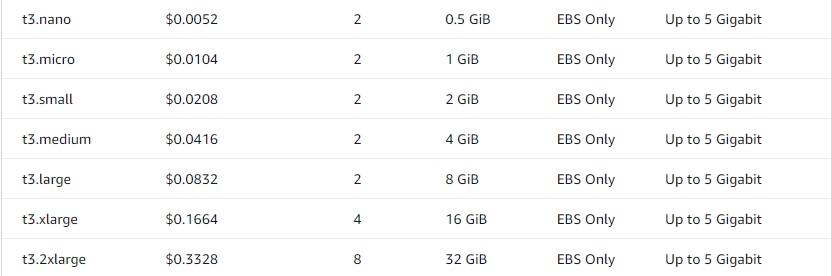
\includegraphics{thesis/img/aws_ec2_pricing.jpg}
        \caption{AWS Prices for EC2 Sampling of Devices}
        \label{fig:ec2-pricing}
    \end{figure}
     This can add up very quickly for large workloads. Edge computing, contrarily, is a far more cost effective method. Since there are no managed services nor massive warehouses of dedicated systems, there is way less overhead that has to be passed on to the end user. This comes with the trade off of a user needing to be much more technically proficient than may be required of an AWS user, but the monetary savings could be very high. 
     
     To estimate the pricing of ECN, one can look at the energy cost of running a laptop in the edge network. A typical laptop consumes 20 watts when idle and 30 watts when operating at 80\% memory usage. The appropriate value to analyze would be the difference between the idle and operating cost, since the idle energy usage is a sunk cost. Converting to kilowatt hours and multiplying by the mid-peak pricing in Ontario, the average cost would be \$0.0011. A user could ask for say \$0.02 per hour of use, and supposing the ECN service took 10\% of this cost as a fee, then the user would profit \$0.0179 per hour. For a job deployer, this cost would be half of renting a t3 medium EC2 instance, resulting in significant savings. 
    
    \section{Environmental}
    \label{sec:environmental}
    The server farms that power the cloud computing services have a massive environmental footprint. There are estimates that the power consumption of all data centres in the world use 200 terawatt per year and account for 2\% of all carbon emissions worldwide. Amazon has been famously very coveted about the specific details of the emissions caused by AWS, however one can estimate the consumption of a single unit with some efficacy. One unit that has similar capacity as the aforementioned EC2 device running at 80\% memory usage is 20 watts. 
    \begin{figure}
        \centering
        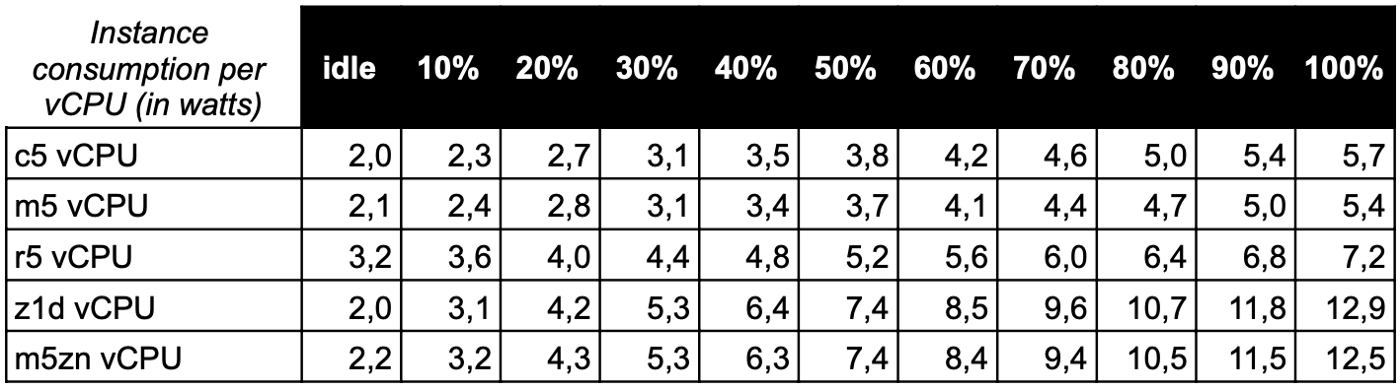
\includegraphics{thesis/img/ec2-energy-consumption.png}
        \caption{AWS Energy Consumption Estimates for EC2 Sampling of Devices}
        \label{fig:ec2-energy}
    \end{figure}
    Edge computing however takes advantage of devices that are already out in the world, and often idling. Granted, there is some increase in power consumption when comparing an idling program to running software at say 80\% capacity, but it would be far less significant than having dedicated servers. In particular, as per the analysis in the economics section the increase for a standard laptop is 10 watts, which would be exactly half of the consumption of the AWS service. The important note about this method of comparison is that the user devices in ECN already exist in the world and are consuming power when idle, so it is indeed appropriate to solely analyze the difference between active and idle usage. 

    
    \section{Social}
    \label{sec:social}
    As discussed in the economics subsection, cloud computing gets expensive. For many with a constrained budget such as scientific researchers or entrepreneurs, cloud computing is prohibitively expensive. For researchers working on groundbreaking cures to illnesses or fantastic advancement in particle physics, cloud computing being too expensive literally slows down innovation on the whole. With the cost savings that come from edge computing comes accessibility to groups that truly can make great use of the technology, and ultimately better society. Take for a example a medical research group studying electron micrographs to understand the 3D structure of proteins. This research helps to understand viruses and can result in figuring out how they spread, and how to treat them more effectively. This reserach is parallelizable, and thus can leverage edge computing to speed up results.
    
    Another factor to consider regarding social impacts of edge computing is the ethics surrounding security and code of ethics with sensitive information. The data used in medical statistical analysis must be scrubbed for private information before being sent out to the ECN, so that people's identities are protected. The Canadian Institutes of Health Research covers the expectations for data integrity. In particular, it is stated that researchers need to vet the places that data is stored so that it is sufficiently protected from loss, theft and corruption. Additionally, researchers need to make sure that identifiable information of study participants are redacted so that identities cannot be recovered from the data. One way these requirements can be satisfied is with encryption of data, and by 
    
\end{document}